\section{ET Model}
\label{sec:ETmodel}

This model is designed to read from file the structure of the ET and to import such Boolean logic structure as a RAVEN model.
The ET must be specified in a specific format: the OpenPSA format (\href{<url>}{https://github.com/open-psa}). 
As an example, the ET of Fig.~\ref{fig:ET} is translated in the OpenPSA format as shown below:

\begin{lstlisting}[style=XML,morekeywords={anAttribute},caption=ET of Fig.~\ref{fig:ET} in OpenPSA format., label=lst:ETmodel]
<define-event-tree name="eventTree">
    <define-functional-event name="ACC"/>
    <define-functional-event name="LPI"/>
    <define-functional-event name="LPR"/>
    <define-sequence name="1"/>
    <define-sequence name="2"/>
    <define-sequence name="3"/>
    <define-sequence name="4"/>
    <initial-state>
        <fork functional-event="ACC">
            <path state="0">
                <fork functional-event="LPI">
                    <path state="0">
                        <fork functional-event="LPR">
                            <path state="0">
                                <sequence name="1"/>
                            </path>
                            <path state="+1">
                                <sequence name="2"/>
                            </path>
                        </fork>
                    </path>
                    <path state="+1">
                        <sequence name="3"/>
                    </path>
                </fork>
            </path>
            <path state="+1">
                <sequence name="4"/>
            </path>
        </fork>
    </initial-state>
</define-event-tree>
\end{lstlisting} 

\begin{figure}
    \centering
    \centerline{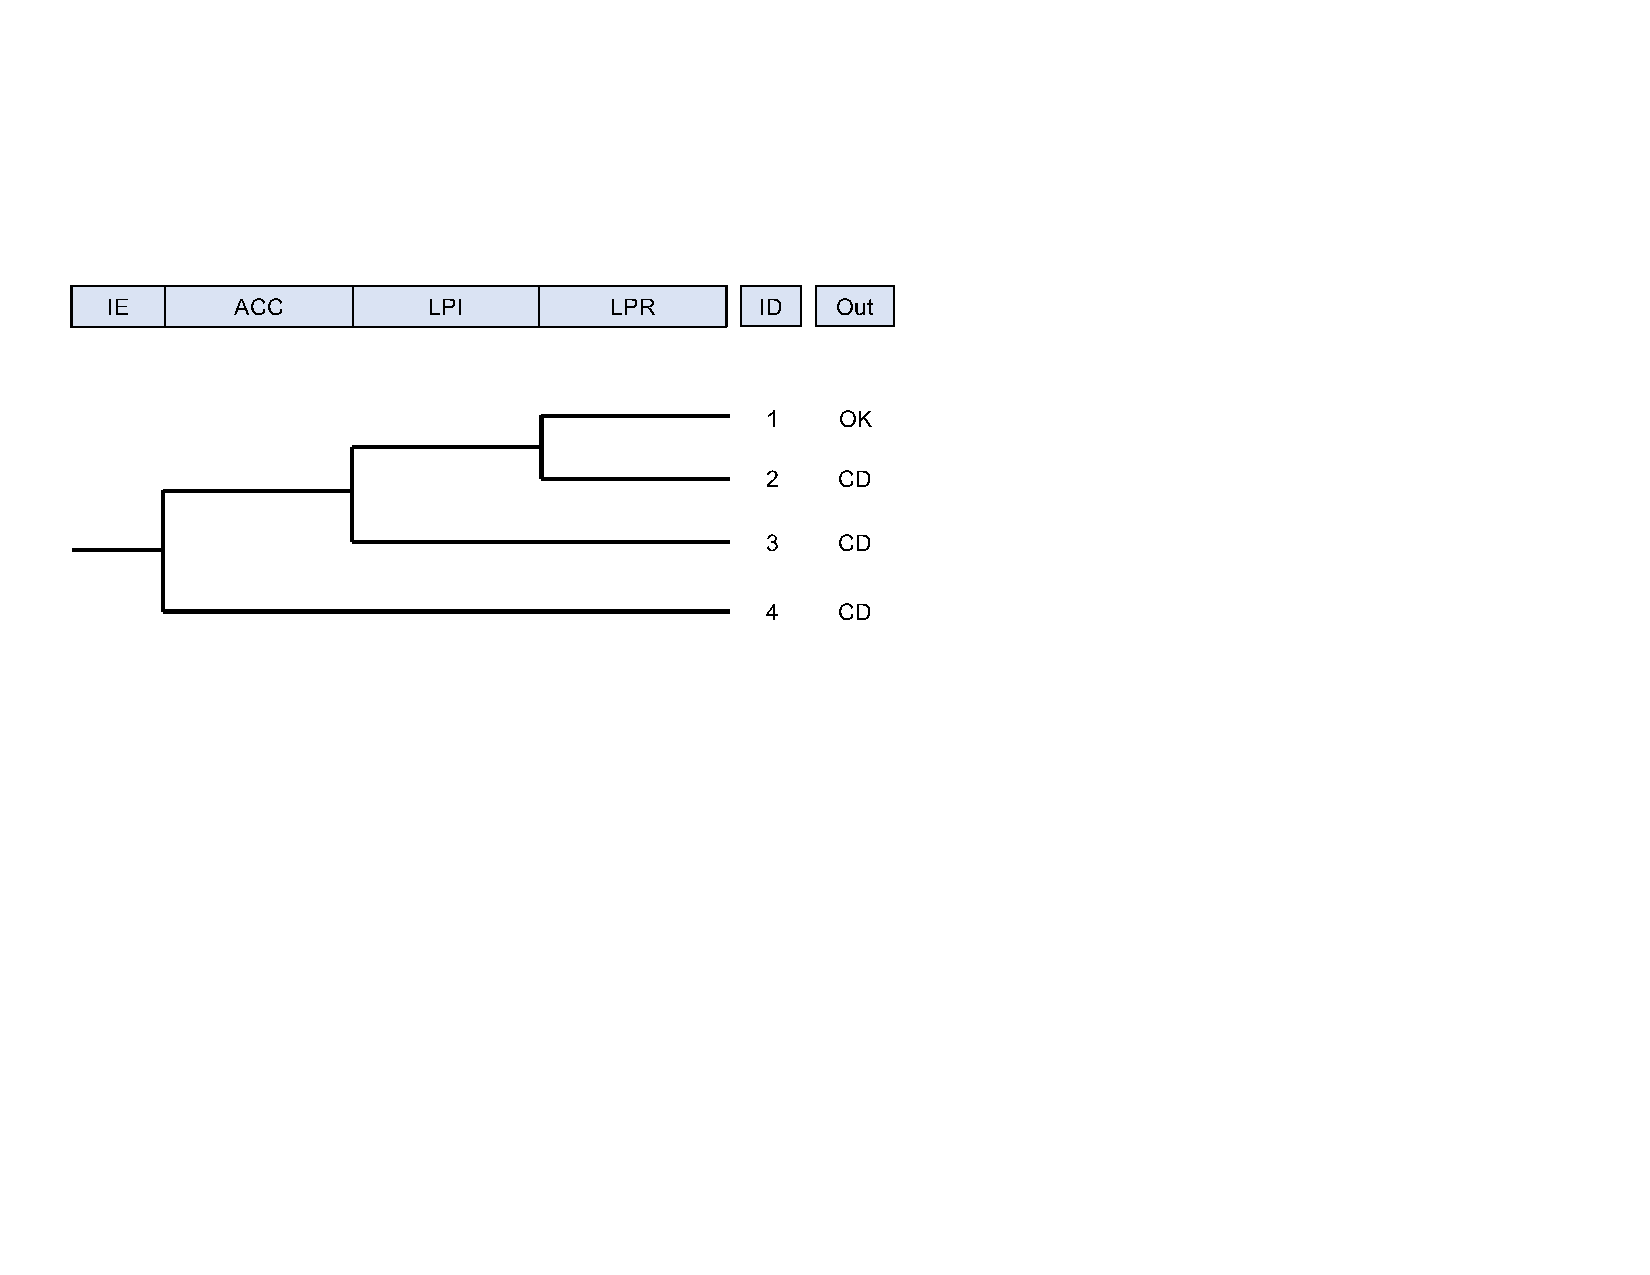
\includegraphics[scale=0.5]{ET.pdf}} 
    \caption{Example of ET.}
    \label{fig:ET}
\end{figure}

The ET of Fig.~\ref{fig:ET} and defined in Listing~\ref{lst:ETmodel} can be defined in the RAVEN input file as follows:
\begin{lstlisting}[style=XML,morekeywords={anAttribute},caption=ET model input example., label=lst:ET_InputExample]
  <Models> 
    ...
    <ExternalModel name="ET" subType="ETmodel">
      <variables>
        statusACC,statusLPI,statusLPR,sequence
      </variables>
      <map var="statusACC">ACC</map>
      <map var="statusLPI">LPI</map>
      <map var="statusLPR">LPR</map>
      <sequenceID>sequence</sequenceID>
    </ExternalModel>
    ...
  </Models>
\end{lstlisting}

All the specifications of the ET model are given in the 
\xmlNode{ExternalModel} block. 
Inside the \xmlNode{ExternalModel} block, the XML
nodes that belong to this models are:
\begin{itemize}
  \item  \xmlNode{variables}, \xmlDesc{string, required parameter}, a list containing the names of both the input and output variables of the model
  \item  \xmlNode{sequenceID},\xmlDesc{string, required parameter}, the name of the alias variable that indicate the branch ID
  \item  \xmlNode{map},\xmlDesc{string, required parameter}, the name ID of the ET branching variable
	  \begin{itemize}
	    \item \xmlAttr{var}, \xmlDesc{required string attribute}, the ALIAS name ID of the ET branching variable
	  \end{itemize}
\end{itemize}

Provided this definition and the ET model of Fig.~\ref{fig:ET} and described in Listing~\ref{lst:ETmodel}, 
the resulting model in RAVEN is characterized by these variables:
\begin{itemize}
	\item Input variables: statusACC, statusLPI, statusLPR
	\item Output variable: sequence
\end{itemize}

\subsection{ET model reference tests}
\begin{itemize}
	\item test\_ETmodel.xml
	\item test\_ETmodel\_TD.xml
\end{itemize}



